\documentclass[10pt, a4paper]{article}
\usepackage[T1]{fontenc}
\usepackage[utf8]{inputenc}
%\usepackage[swedish]{babel}
\usepackage{ifpdf}
\usepackage[parfill]{parskip}
\usepackage{graphicx}
\usepackage{fancyvrb}   % For source code listing.
\fvset{tabsize=4}       % Tabstop is 4 spaces.
\fvset{fontsize=\small} % Small fonts for source code.

\title{EDA031 Project - News System}
%\date{}
\author{
	\begin{tabular}{l l}
		Erik Westrup & \texttt{<ada09ewe@student.lu.se>}\\
		Joachim Nelson & \texttt{<ada08jne@student.lu.se>} \\ % TODO rätt mail?
		Oscar Olsson & \texttt{<ada09ool@student.lu.se>}
	\end{tabular}
}

\begin{document}

\begin{titlepage}
\maketitle
\thispagestyle{empty}	% No page number on title page.
\end{titlepage}
%\setcounter{page}{2}

\section{EDA031 Project - News System}

\subsection{Detailed description of desing and UML}
\begin{figure}[hbt]
\begin{center}
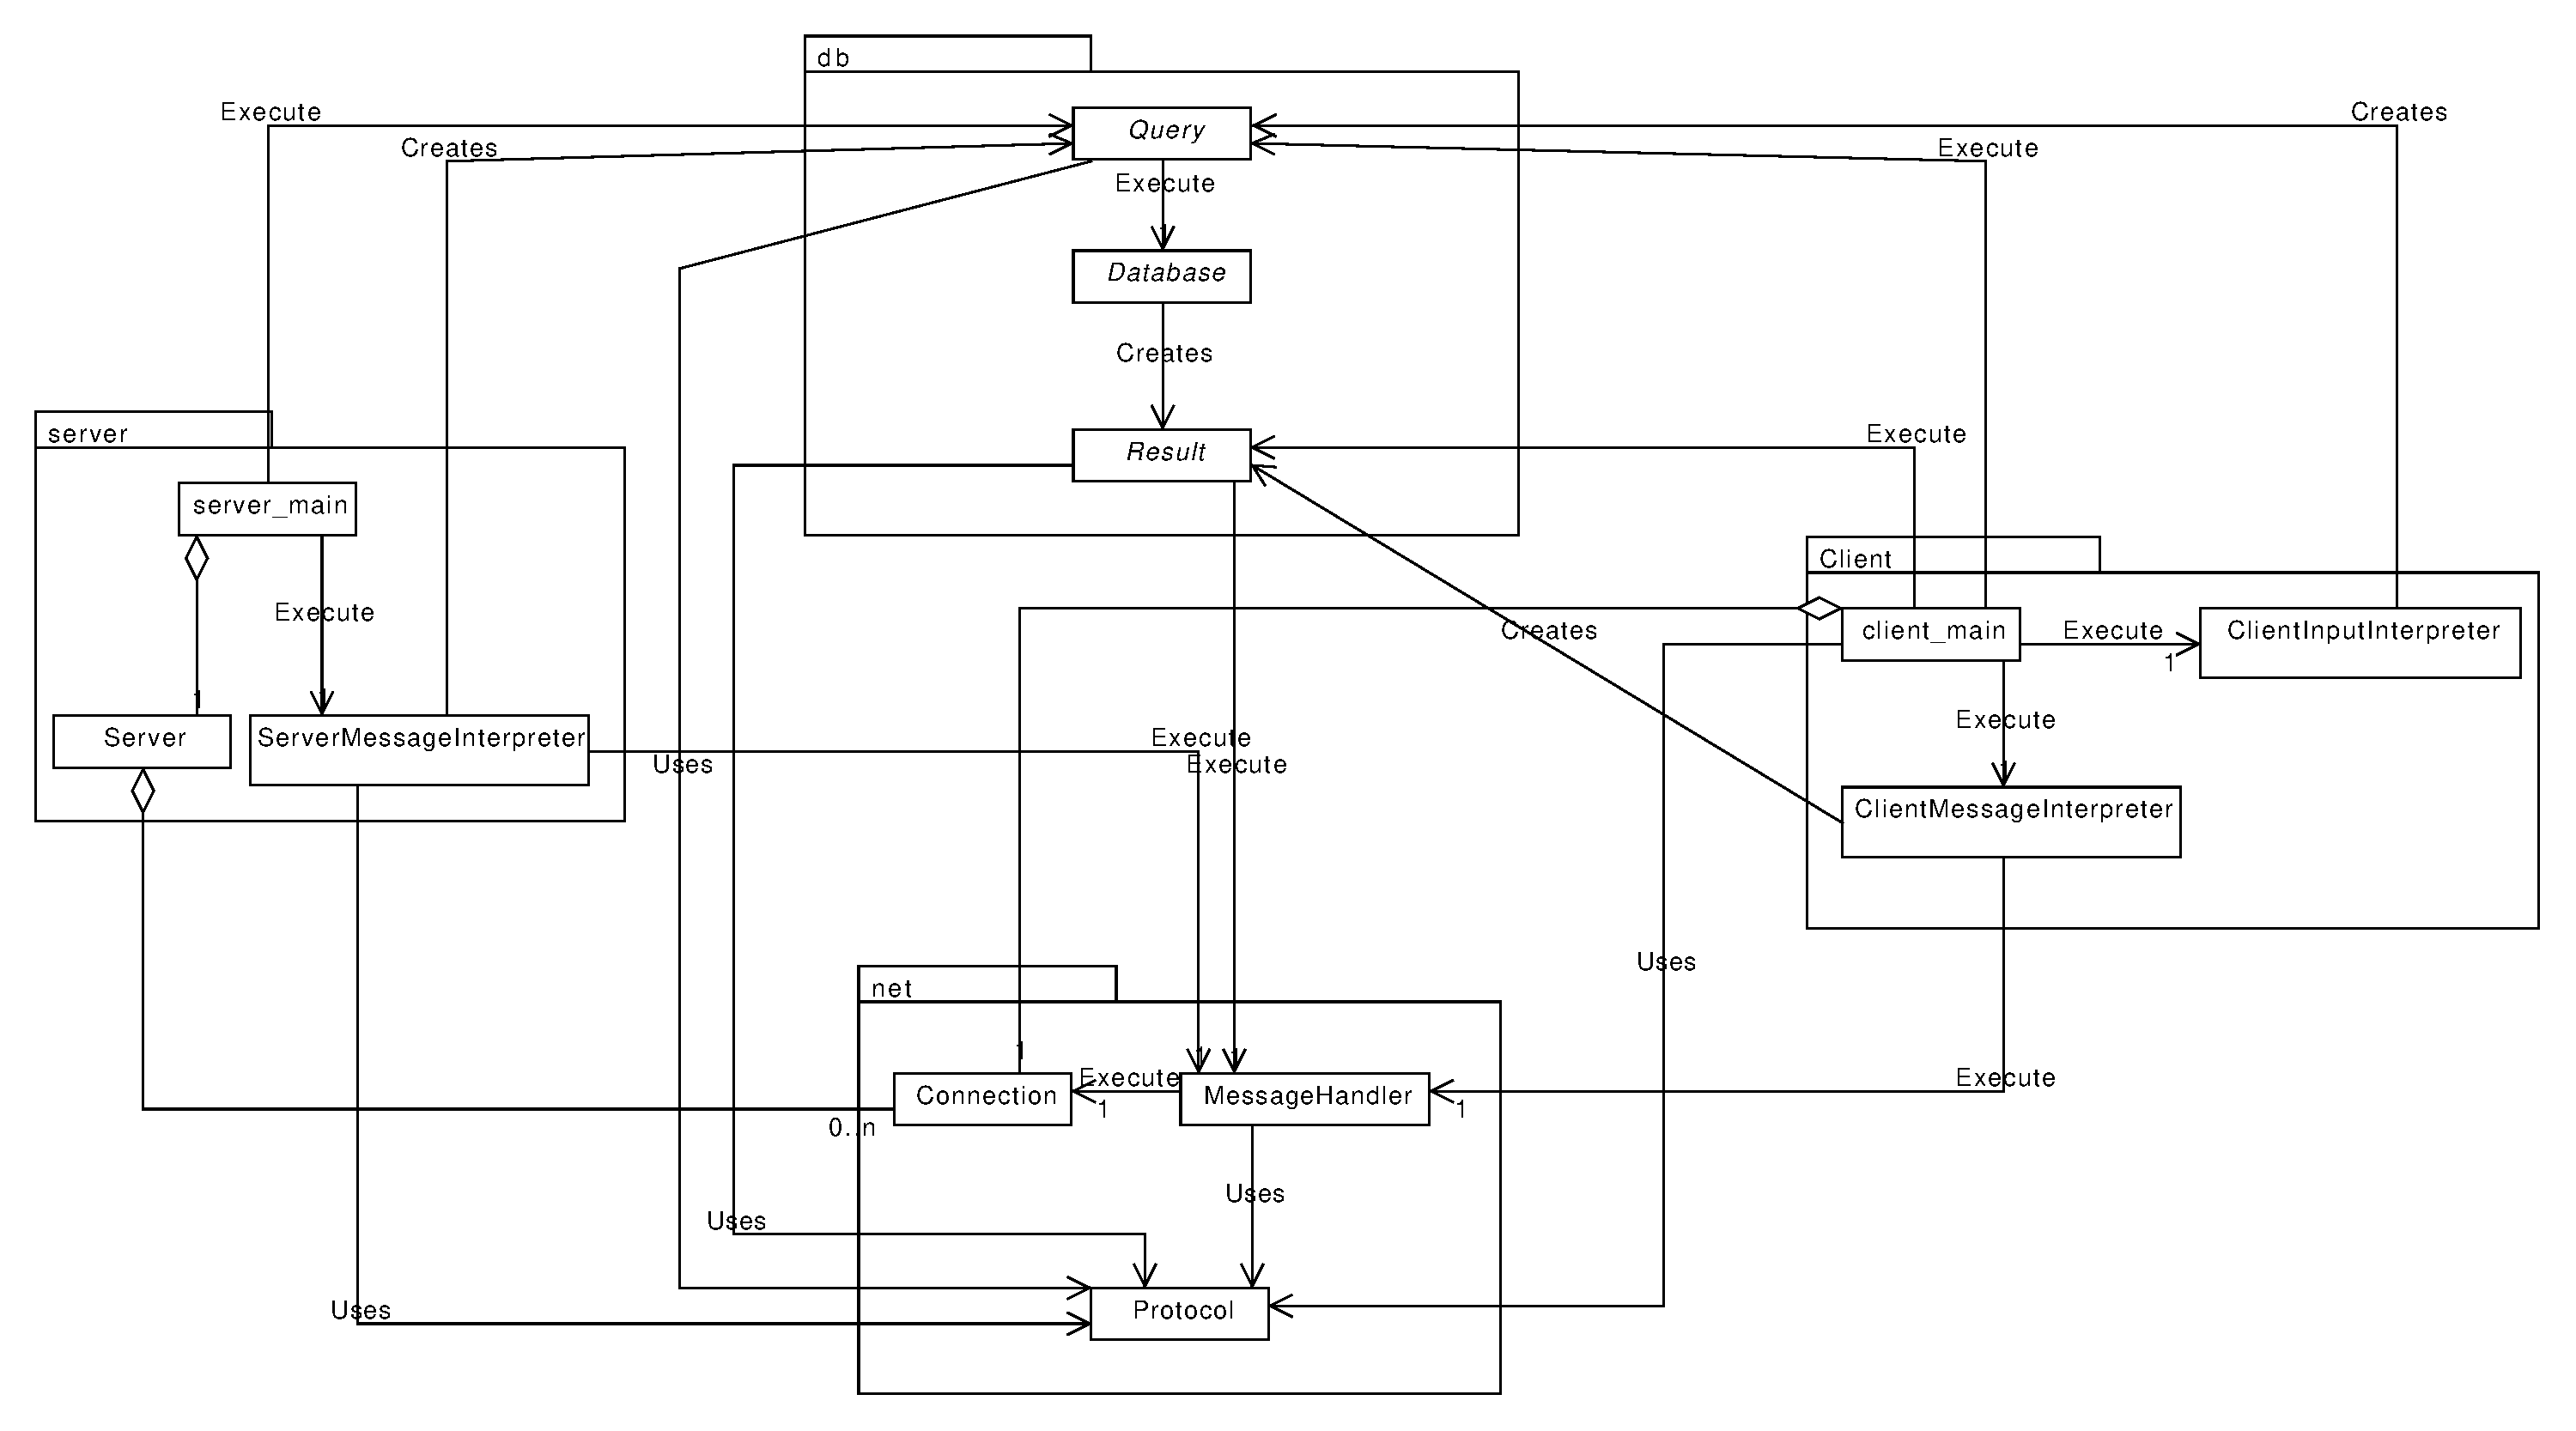
\includegraphics[scale=0.3]{uml.pdf}
\end{center}
\label{UML}
\caption{An UML diagram describing the project.}
\end{figure}

\subsection{Communication, flow-chart}

\subsection{Conclusion}

\subsubsection{Implemented requirements}

\subsubsection{Unsolved problems}

\subsubsection{Missing features}

\subsubsection{Suggestions}

\emph{\cite{dummy+ref}} 
\newpage
\bibliographystyle{plain}
\bibliography{references}
\end{document}

%\begin{figure}[hbt]
%\begin{center}
%\includegraphics[scale=0.4]{img/pic1.png}
%\end{center}
%\label{LABEL}
%\caption{DESCRIPTION text.}
%\end{figure}
%\clearpage

%\VerbatimInput{src/prog1.c}
